The results of model independent limits are interpreted in terms of limits
computed for squark pair production with $\squarkprod$ in a SUSY compressed
scenario. The sensitivity to these models is estimated by performing a global
signal plus background fit that includes the $\crele$, $\crwmn$, $\crzmm$
control regions, the signal regions and all the systematic uncertainties. The
expected limits are derived with the same procedure but by replacing the data
with the background prediction.

Figure~\ref{fig:expected_observed} shows the result limits on the SUSY
compressed squark--neutralino model for the Run~II 2015 data. This is the result
of the shape fit with a luminosity of $3.2~\ifb$ with all theoretical signal
systematic uncertainties included in the observed and expected exclusion contour
and using the $\crele$, $\crwmn$, $\crzmm$ control regions. The theoretical
uncertainty on the signal cross section is used to derive the uncertainty on the
observed limit.

Models with a mass gap of $\Delta m = 5$~GeV between the squark and the
neutralino mass can be excluded up to squark masses of 608~GeV. For larger mass
gap of $\Delta m = 25$~GeV, squark masses up to 532~GeV are also excluded. The
results of this study are combined with the more general SUSY searches adding
sensitivity to the region close to the diagonal (dashed line) in
\cref{fig:susy_exclusion}.


\begin{figure}[!h]
  \centering
    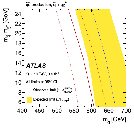
\includegraphics[width=.8\linewidth]{expected_observed}
    \caption{Expected and observed limits on the SUSY compressed models using
      the Run~2 2015 data, in the plane defined by the squark mass on the
      $x$-axis and the mass difference between the squark and lightest
      neutralino mass on the $y$-axis. All experimental and theoretical
      systematic uncertainties are included.}
\label{fig:results:susy:compressed_observed}
    \label{fig:expected_observed}
\end{figure}
%%% Local Variables:
%%% mode: latex
%%% TeX-master: "../search_for_DM_LED_with_ATLAS"
%%% End:
